
%%%%%%%%%%%%%%%%%%%%%%% file typeinst.tex %%%%%%%%%%%%%%%%%%%%%%%%%
%
% This is the LaTeX source for the instructions to authors using
% the LaTeX document class 'llncs.cls' for contributions to
% the Lecture Notes in Computer Sciences series.
% http://www.springer.com/lncs       Springer Heidelberg 2006/05/04
%
% It may be used as a template for your own input - copy it
% to a new file with a new name and use it as the basis
% for your article.
%
% NB: the document class 'llncs' has its own and detailed documentation, see
% ftp://ftp.springer.de/data/pubftp/pub/tex/latex/llncs/latex2e/llncsdoc.pdf
%
%%%%%%%%%%%%%%%%%%%%%%%%%%%%%%%%%%%%%%%%%%%%%%%%%%%%%%%%%%%%%%%%%%%

\let\origvec\vec
\documentclass[runningheads,a4paper]{llncs}



%******Figure and Table Package
\usepackage{color}
\usepackage{amsfonts}
%\usepackage{ulem}    % underline/strikethrough/wave lines
\usepackage{graphicx}  % figures
\usepackage{tabularx}
\usepackage{subfigure}
\usepackage{figlatex}
\usepackage{graphics}
\usepackage{caption}
%\usepackage{subcaption}
\usepackage{multirow}
\usepackage{tikz}
\usetikzlibrary{shapes,shadows,calc}
\usepgflibrary{arrows}


%**********Math package

\let\springervec\vec
\let\vec\origvec
\usepackage{amsmath}
\usepackage{amssymb}
\usepackage{latexsym}
\setcounter{tocdepth}{3}
\usepackage{mathpartir}


%---Algorithm
\renewcommand{\thechapter}{\Roman{chapter}}
\renewcommand{\thesection}{\arabic{section}}

\usepackage[chapter]{algorithm}
\usepackage{algorithmicx}
\usepackage{algpseudocode}

\renewcommand{\thealgorithm}{\arabic{chapter}.\arabic{algorithm}} 


%----Graph
\usepackage{tikz,mathpazo}  % This package is used to draw the figure
\usetikzlibrary{shapes.geometric, arrows}
\usetikzlibrary{positioning,shapes.geometric}

\usepackage{palatino}
\usetikzlibrary{shapes.geometric, arrows}
\usepackage{xcolor}
\usetikzlibrary{shapes,arrows,chains}

%----- pNet macros package
\usepackage{epsfig,enumitem}
\newcommand{\TODO}[1]{\textcolor{red}{\textbf{[TODO:#1]}}}
\newcommand{\NOTE}[1]{\textcolor{blue}{\textbf{[NOTE:#1]}}}
\newcommand{\ERIC}[1]{\textcolor{blue}{#1}}
\definecolor{darkgreen}{rgb}{0.1, 0.5, 0.1}
\newcommand{\coloncolon}{{:\hspace{-.2ex}:}}
\makeatletter
\newcommand{\raisemath}[1]{\mathpalette{\raisem@th{#1}}}
\newcommand{\raisem@th}[3]{\raisebox{#1}{$#2#3$}}
\makeatother

\usepackage{macrospNets}


\newcommand{\Simon}{\\\hfill\mdash Simon}

\newcommand{\noteSB}[2][color=green!40, size=\tiny]{\todo[#1]{{#2}\Simon}}
\newcommand{\noteSBin}[2][inline,color=green!40]{\todo[#1]{{#2}\Simon}}
\newcommand{\todoSB}[2][color=green!40, size=\tiny]{\todo[#1]{\textbf{To-do Simon:} {#2}}}
\newcommand{\todoSBin}[2][inline,color=green!40]{\todo[#1]{\textbf{To-do Simon: } {#2}}}
\newcommand{\Ludo}{\\\hfill\mdash Ludo}
\newcommand{\noteLH}[2][color=orange!40, size=\tiny]{\todo[#1]{{#2}\Ludo}}
\newcommand{\noteLHin}[2][inline,color=orange!40]{\todo[#1]{{#2}\Ludo}}
\newcommand{\todoLH}[2][color=orange!40, size=\tiny]{\todo[#1]{\textbf{To-do Ludo:} {#2}}}
\newcommand{\todoLHin}[2][inline,color=orange!40]{\todo[#1]{\textbf{To-do Ludo: } {#2}}}

\newcommand{\noteIn}[2][inline,color=black!20]{\todo[#1]{{#2}}}

\newcommand{\add}[2][Added]{\todo[color=blue!20, size=\tiny]{#1}{\color{blue}#2}}
%% \newcommand{\remove}[2][Removed]{\todo[color=red!20, size=\tiny]{#1}}
\newcommand{\remove}[2][Removed]{\todo[color=red!20, size=\tiny]{#1}{\color{red}\st{#2}}}
\newcommand{\removeIn}[2][Removed]{\todo[color=red!10, inline]{{\color{red}#2}#1}}
%% \newcommand{\replace}[3][Replaced]{\todo[color=blue!20, size=\tiny]{#1}{\color{blue}#3}}
\newcommand{\replace}[3][Replaced]{\todo[color=blue!20, size=\tiny]{#1}{\color{blue}#3}{\color{red}\st{#2}}}

\newcommand{\addSB}[1]{\add[Added by Simon]{#1}}
\newcommand{\removeSB}[1]{\remove[Removed by Simon]{#1}}
\newcommand{\removeSBin}[1]{\removeIn[Removed by Simon]{#1}}
\newcommand{\replaceSB}[2]{\replace[Replaced by Simon]{#1}{#2}}

\newcommand{\defn}[1]{Def.~\ref{defn:#1}}
\newcommand{\defntwo}[2]{Defs~\ref{defn:#1} and \ref{defn:#2}}
\newcommand{\fig}[1]{Fig.~\ref{fig:#1}}
\newcommand{\Fig}[1]{Figure~\ref{fig:#1}}
\newcommand{\figs}[2]{Fig.~\ref{fig:#1} and~\ref{fig:#2}}
\newcommand{\tab}[1]{Tab.~\ref{tab:#1}}
\newcommand{\eq}[1]{(\ref{eq:#1})}
\newcommand{\res}[1]{(\ref{res:#1})}
\newcommand{\ex}[1]{Ex.~\ref{ex:#1}}
\newcommand{\exs}[2]{Ex.~\ref{ex:#1} and~\ref{ex:#2}}
\newcommand{\secn}[1]{Sect.~\ref{secn:#1}}
\newcommand{\rem}[1]{Note~\ref{rem:#1}}
\newcommand{\lem}[1]{Lem.~\ref{lem:#1}}
\newcommand{\cor}[1]{Cor.~\ref{cor:#1}}
\newcommand{\thm}[1]{Th.~\ref{thm:#1}}
\newcommand{\axs}[1]{Ax.~\ref{ax:#1}}
% \newcommand{\ax}[2]{\ref{ax:#1}.\ref{ax:#1:#2}}
\newcommand{\ax}[1]{Ax.~\ref{ax:#1}}
\newcommand{\prop}[1]{Prop.~\ref{prop:#1}}
\newcommand{\alg}[1]{Alg.~\ref{alg:#1}}
\newcommand{\asmp}[1]{Ass.~\ref{asmp:#1}}

% %%%%%%%%%%%%%%%%%%%%%

\newcommand{\cA}{\ensuremath{\mathcal{A}}}
\newcommand{\fA}{\ensuremath{\mathsf{A}}}
\newcommand{\sA}{\ensuremath{\mathbb{A}}}
\newcommand{\cB}{\ensuremath{\mathcal{B}}}
\newcommand{\fB}{\ensuremath{\mathsf{B}}}
\newcommand{\sB}{\ensuremath{\mathbb{B}}}
\newcommand{\cC}{\ensuremath{\mathcal{C}}}
\newcommand{\sC}{\ensuremath{\mathbb{C}}}
\newcommand{\cD}{\ensuremath{\mathcal{D}}}
\newcommand{\fD}{\ensuremath{\mathsf{D}}}
\newcommand{\sD}{\ensuremath{\mathbb{D}}}
\newcommand{\cE}{\ensuremath{\mathcal{E}}}
\newcommand{\sE}{\ensuremath{\mathbb{E}}}
\newcommand{\cF}{\ensuremath{\mathcal{F}}}
\newcommand{\cG}{\ensuremath{\mathcal{G}}}
\newcommand{\cH}{\ensuremath{\mathcal{H}}}
\newcommand{\cI}{\ensuremath{\mathcal{I}}}
\newcommand{\sI}{\ensuremath{\mathbb{I}}}
\newcommand{\cM}{\ensuremath{\mathcal{M}}}
\newcommand{\cN}{\ensuremath{\mathcal{N}}}
\newcommand{\sN}{\ensuremath{\mathbb{N}}}
\newcommand{\cP}{\ensuremath{\mathcal{P}}}
\newcommand{\sP}{\ensuremath{\mathbb{P}}}
\newcommand{\cQ}{\ensuremath{\mathcal{Q}}}
\newcommand{\sQ}{\ensuremath{\mathbb{Q}}}
\newcommand{\cR}{\ensuremath{\mathcal{R}}}
\newcommand{\sR}{\ensuremath{\mathbb{R}}}
\newcommand{\cS}{\ensuremath{\mathcal{S}}}
\newcommand{\sS}{\ensuremath{\mathfrak{S}}}
\newcommand{\cT}{\ensuremath{\mathcal{T}}}
\newcommand{\fT}{\ensuremath{\mathsf{T}}}
\newcommand{\sT}{\ensuremath{\mathbb{T}}}
\newcommand{\cV}{\ensuremath{\mathcal{V}}}
\newcommand{\fV}{\ensuremath{\mathsf{V}}}
\newcommand{\sV}{\ensuremath{\mathbb{V}}}
\newcommand{\sZ}{\ensuremath{\mathbb{Z}}}

\newcommand{\mdash}[1][]{---#1}
\newcommand{\ndash}{--}
\newcommand{\ie}[1][\ ]{i.e.#1}
\newcommand{\etc}[1][\ ]{etc.#1}
\newcommand{\eg}[1][\ ]{e.g.#1}
\newcommand{\cf}[1][\ ]{cf.#1}
\newcommand{\wrt}[1][\ ]{w.r.t.#1}
\newcommand{\resp}[1][\ ]{resp.#1}

\newcommand{\bydef}[1]{\ensuremath{\stackrel{\mathit{\scriptscriptstyle def}}{#1}}}
\newcommand{\suchthat}{\ensuremath{\,|\,}}
\newcommand{\rightsuchthat}{\ensuremath{\,\right|\,}}
\newcommand{\leftsuchthat}{\ensuremath{\,\left|\,}}
\newcommand{\setdef}[2]{\ensuremath{\{{#1}\,|\,{#2}\}}}
\newcommand{\setdefb}[2]{\ensuremath{\bigl\{{#1}\,\bigl|\,{#2}\bigr.\bigr\}}}
\newcommand{\Setdef}[2]{\ensuremath{\Big\{{#1}\,\Big|\,{#2}\Big\}}}
\newcommand{\goesto}[2][]{\ensuremath{\xrightarrow[#1]{#2}}}
\newcommand{\notgoesto}[2][]{\ensuremath{\not\xrightarrow[#1]{\ \,#2}}}
\newcommand{\non}[1]{\ensuremath{\overline{#1}}}

\newcommand{\true} {\ensuremath{\mathtt{t\!t}}}
\newcommand{\false}{\ensuremath{\mathtt{f\!f}}}
\newcommand{\noop} {\ensuremath{\emptyset}} % \mathsf{skip}

\newcommand{\ordbool}{\ensuremath{\sB^{<}}}
\newcommand{\data}{\ensuremath{\sD}}
\newcommand{\signature}{\ensuremath{\Sigma}}
\newcommand{\variables}{\ensuremath{\cV}}
\newcommand{\Talg}{\ensuremath{\cT_{\signature,\variables}}}
\newcommand{\actions}[1]{\ensuremath{\cA_{#1}}}
\newcommand{\guards}[1]{\ensuremath{\ordbool_{#1}}}
\newcommand{\exprs}[1]{\ensuremath{\sE_{#1}}}
\newcommand{\boolexprs}[1]{\ensuremath{\sB_{#1}}}
\newcommand{\assigns}[1]{\ensuremath{\sA_{#1}}}
\newcommand{\valuations}[1]{\ensuremath{\data^{#1}}}
\newcommand{\val}[3][]{\ensuremath{#1{\sigma}^{#2}_{#3}}}

\newcommand{\filter}[2][]{\ensuremath{\pi_{#1}({#2})}}

\newcommand{\primeit}[1]{#1'}
\newcommand{\doubleprimeit}[1]{#1''}


\newcommand{\export}[1][]{\ensuremath{\varepsilon_{#1}}}
\newcommand{\valdiff}[2]{\ensuremath{#1 \triangle #2}}
\newcommand{\supp}[1]{\ensuremath{\mathrm{supp}(#1)}}
\newcommand{\semopen}[1]{\ensuremath{[{#1}]}}
\newcommand{\semclosed}[1]{\ensuremath{\llbracket{#1}\rrbracket}}
\newcommand{\reachable}[1]{\ensuremath{\mathit{reachable}({#1})}}
\newcommand{\IMextend}[2]{\ensuremath{#1 \ltimes #2}}
\newcommand{\arcomp}{\oplus}
\newcommand{\arequiv}{\equiv}
\newcommand{\Arcomp}{\Bigoplus}
\newcommand{\expmix}{\wedge}
\newcommand{\order}{\leqslant}





\usepackage{url}


\urldef{\mailtengfei}\path|{tengfeili2018}@gmail.com| 
\urldef{\mailinria}\path|{eric.madelaine}@inria.fr|      
\newcommand{\keywords}[1]{\par\addvspace\baselineskip
\noindent\keywordname\enspace\ignorespaces#1}

\begin{document}

\mainmatter  % start of an individual contribution

% first the title is needed
\title{Model Checking for Open Concurrent Systems}

% a short form should be given in case it is too long for the running head
\titlerunning{Lecture Notes in Computer Science: Authors' Instructions}

% the name(s) of the author(s) follow(s) next
%
% NB: Chinese authors should write their first names(s) in front of
% their surnames. This ensures that the names appear correctly in
% the running heads and the author index.
%
\author{Tengfei?Li
\and Eric?Madelaine \and *
}
%
\authorrunning{Lecture Notes in Computer Science: Authors' Instructions}
% (feature abused for this document to repeat the title also on left hand pages)

% the affiliations are given next; don't give your e-mail address unless you accept that it will be published


\institute{
%\mailtengfei\\
%\mailinria\\
}

%
% NB: a more complex sample for affiliations and the mapping to the
% corresponding authors can be found in the file "llncs.dem"
% (search for the string "\mainmatter" where a contribution starts).
% "llncs.dem" accompanies the document class "llncs.cls".
%

\toctitle{Lecture Notes in Computer Science}
\tocauthor{Authors' Instructions}
\maketitle


\begin{abstract}

The verification of concurrent systems, especially concurrent systems with data, have been researched for many years. However, the composition of concurrent systems have not been solved well. The major problem is ...

\keywords{ pM$\mu$\quad $pMG $\quad pLTS }
\end{abstract}


\section{Introduction}
% no \IEEEPARstart

\section{Use-case: The BIP Failure-Timer architecture}\label{Sec2:usecase}



\TODO{Describe here the full Failure-Timer architecture, as taken from the Avocs paper, including an informal presentation of the original BIP system, its full translation into a pNet system (pLTSs and pNet nodes), and the generated Open Automaton}
\NOTE{All figures are already available from the Avocs paper sources.}

The BIP architecture includes two kinds of components, coordinator component and operand component. The operand component just has some ports used to communicate with other component. While the coordinator components don't only have some ports, but they include a parameterised labelling transition system (pLTS) in them. In a pLTS, some nodes and edges between these nodes are built to describe the coordinator component. In a pLTS, a node denotes the state of the component, while a edge means the transition from one state to another. Specifically, a port in a coordinator component is used to label a transition, and the number of transitions is the same as that of ports. 


\begin{figure}[ht]
  \centering
  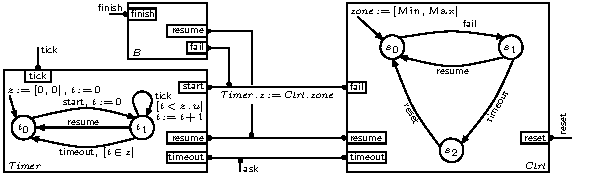
\includegraphics[width=0.8\columnwidth]{figures/BIPspec-ArchFailureTimerMax-v3.pdf}
  \caption{The BIP specification of the Failure Monitor architecture}
  \label{schema:ArchFailure:BIP}
\end{figure}

Fig.~\ref{schema:ArchFailure:BIP} shows the BIP specification of the Failure-Timer architecture from~\cite{xudong2017smt}.  $Timer$ and $Controller$ are the coordinator components, and $B$ is an operand component. $Timer$ has four ports, like $start$, $tick$, $resume$ and $timeout$, and these ports are labelling the transitions between the two states $t_{0}$, and $t_{1}$. And $Ctrl$ has four ports, like $fail$, $reset$, $resume$ and $timeout$, and these ports are labelling the transitions between the three states $s_{0}$, $s_{1}$ and $s_{2}$. The operand component $B$ has three ports $resume$, $fail$ and $finish$.


\begin{figure}[ht]
  \centering
  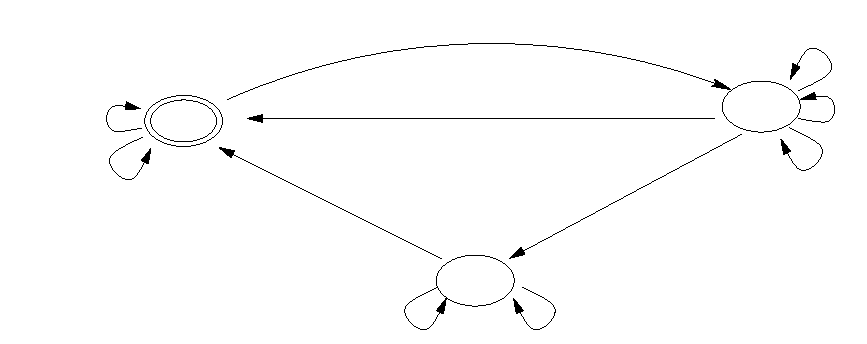
\includegraphics[width=0.8\columnwidth]{figures/FailureTimerOA.pdf}
  \caption{The Open Automaton of the Failure Monitor architecture}
  \label{schema:ArchFailure:OA}
\end{figure}


In~\cite{xudong2017smt}, an approach is present to unfold the open pNet to open automata. Fig.~\ref{schema:ArchFailure:OA} shows the open automaton unfolded from the Failure-Timer architecture in Fig~\ref{schema:ArchFailure:BIP}. The state is the composition of the states of each pLTS in the coordinator component, while the transition is labelled with a composition of the corresponding action in each component. For example, in the BIP specification, $Timer.start$ synchronises with $Ctrl.fail$, because there is a connector between the two ports. When occurrence of the transition $s_{0}\xrightarrow{fail}s_{1}$ will trigger the execution of the transition $t_{0}\xrightarrow{start, t:=0}t_{1}$. At the same time, the port $Ctrl.fail$ will synchronise with $B.fail$. The connected ports in Failure-Timer architecture form a synchronisation vector. The synchronisation will return to a special action, which can be used to label a transition.


\section{Describing pLTS}

\subsection{pLTS}

In a pLTS, each state is composed of a set of $\mathit{state\ variables}$, and a transition is defined between two states. A triple with $\mathit{parameterised\ action}, \mathit{guard}$ and $\mathit{assignment}$ consists of the labelling function of the transition.

\subsubsection{Definition of pLTS}
We define pLTS as a triple: $pLTS\triangleq\ll S, s_{0}, \rightarrow \gg$ where:
\begin{itemize}
	\item $S$ is a set of states, and $s_{0}\in S$ is the initial state.
	\item $\rightarrow \subseteq S\times L\times S$ is the transition relation, with $L$ the set of labels of form $\langle\alpha, e_{b}, (x_{j} := e_{j})^{(j\in J)}\rangle$, where $\alpha\in A_{V}$ is a parameterised action, $e_{b}\in B_{V}$ is a guard, and expression $E_{P}\cup A_{P}$ are assigned to $x_{j}$. If $s\xrightarrow{\langle\alpha, e_{b}, (x_{j}:=e_{j})^{j\in J}\rangle}s' \in \rightarrow$, then $vars(e_{b})\subseteq vars(s)\cup vars(\alpha)$, and $\forall j\in J. vars(e_{j})\subseteq vars(s)\wedge x_{j}\in vars(s')$.
\end{itemize}

\begin{figure}[ht]
  \centering
  \includegraphics[width=0.8\columnwidth]{figures/TimerpLTS.eps}
  \caption{The pLTS of the Timer component}
  \label{schema:Timer:pLTS}
\end{figure}



\subsection{Property Language}

A major difference of pLTS from other concurrent systems is the parameterised action. Basic MCL\cite{radu2008mcl} extends action in modal $\mu$-calculus with data variables, so it suits for describing the property of open concurrent systems. We define a subset of basic MCL, named parameterised modal $\mu$-calculus (pM$\mu$), to describe the properties of pLTS. Tab.~\ref{mcl} shows the syntax of pM$\mu$.

\begin{table}
	%	\multirow{2}{*}{Algorithme}
	\setlength\tabcolsep{18pt}% default value is 6pt 
	\centering 
	\caption{Syntax of the pM$\mu$} 
	\label{mcl}
	\begin{tabular}{>{\bfseries}c| c } 
		\hline 		
	Action formula 	&     $\alpha ::= \{c(arg_{1}, ..., arg_{n})\mid arg_{i}=?x\mid\ !e\mid \tau\}$                  \\
	& $|\ \neg\alpha \ |\ \alpha_{1}\vee\alpha_{2}\ |\ \alpha_{1}\wedge\alpha_{2}$   \\ 	\hline 
		
	State formula 	&  $\varphi ::= p \mid X \mid \neg\varphi \mid \varphi_{1}\wedge\varphi_{2}\ |\ \varphi_{1}\vee\varphi_{2} \ |\ [\alpha]\varphi \ |\ \langle\alpha\rangle\varphi$ \\ 
	& $\exists x_{i}\varphi\ |\ \forall x_{i}\varphi\ |\ \mu X(e_{i}/x_{i})\varphi\ |\ \nu X(e_{i}/x_{i})\varphi$	\\ \hline 
	\end{tabular} 
\end{table} 
 
 where, $c$ is an action name expressing the communication port. $arg_{i}$ is a list of arguments, and each $arg_{i}$ is either a send expression $!e$, a receive variable $?x$ or a silent action $\tau$. An action $\alpha$ is a parameterised action $c(arg_{i})$. $p$ is an atomic proposition and $X$ is a set of variables. $\neg$, $\vee$ and $\wedge$ are respectively negation, disjunction and conjunction operator on action formula and state formula. $[\alpha]\varphi$ expresses "whenever an action $\alpha$ happens, we will do $\varphi$", and $\langle\alpha\rangle$ expresses "an action $\alpha$ takes effective, we will do $\varphi$". $x_{i}\in X$ is a free variable bound in state formula $\varphi$. $\mu$ and $\nu$ are respectively the minimum fixed point and the maximum fixed point.\TODO{Tengfei: Must more explaination}\NOTE{Done}


We employ the case study from timer component~\cite{mavridou2016architectrue}. A liveness property defines that good thing finally happens. In this case study, intuitively the timer finally returns to the initial state after some execution steps. The property can be expressed by a pM$\mu$ formula:

\begin{equation}\label{formula1}
	\langle start?M\rangle\mu X(M/t)(\langle timeout\rangle true \vee \langle tick\rangle X(t-1/t))
\end{equation}


\ERIC{this description is too operational (like a state machine), I would like a more logical description of the formula. One way is to use the vocabulary of ``Specification patterns'', like ``it is possible'', ``it is mandatory'', ``do something until some condition'', etc}

At first, a $start$ occurs with receiving a value $M$, and then it is mandatory to enters a loop with an assignment $t := M$.  In the loop $\mu$, it is possible for the timer to return true until an action $timeout$ happens, and it is done. Or it will continue the loop with decreasing the value $t$ by one when the $tick$ again.


\subsection{pMG}

Modal graph is present by Lin\cite{lin2001modal}. We consider a variant of modal graph, parameterised modal graph (pMG), as the graphical version of pM$\mu$. We define a collection of modal operators as $ModOp = \{[\alpha], \langle\alpha\rangle\}$. A pMG is a directed graph $\langle N, E, L_{N}, n_{0}\rangle$, where
\begin{itemize}
	\item $N$ is a set of nodes.
	\item $E \subseteq N\times N$ is the set of edges.
	\item $L_{N} = (L_{V}, L_{O}, L_{D})$ associates each node $n\in N$ a set of variables $L_{V}(n)$, an operator $L_{O}(n)\in\{\wedge, \vee, \forall x, \exists x, \theta\}\cup ModOp \cup BExp$, and a depth $L_{D}(n)$ which is a natural number.
	\item $n_{0} \in N$ is the root of a pMG.
\end{itemize}



\subsection{Transformation from pM$\mu$ to pMG}

 Given a pM$\mu$ formula $F$ and a pMG, we define a node as a subformula $\phi$ of $F$. The edge between two nodes will be the transition from a subformula to another subformula. The transformation rules can be seen in Lin's paper~\cite{lin2001modal}. The rules take a pM$\mu$ formula as the input and generate a pMG. 

In the case study, the liveness property is present as Formula~\ref{formula1}. The alternation depth is 1, because there is only one $\mu$ operator. The corresponding modal graph is shown as follows:


\begin{figure}
\centering
	\begin{tikzpicture}[->, shorten >=2pt, >=stealth, node distance=1.2cm,
	noname/.style={ellipse, minimum width=1.5em, minimum height=1.5em, draw}]
	\node[noname] (1)                                            				 	{$t_{1}$};
	\node[noname] (2) [right=of 1]                               				 	{$t_{2}$};
	\node[noname] (3) [right=of 2]                              				 	{$t_{3}$};
	\node[noname] (4) [node distance=0.5cm and 2cm, above right=of 3]    {$t_{4}$};
	\node[noname] (5) [right=of 4]                                					{$t_{5}$};
	\node[noname] (6) [node distance=0.5cm and 2cm, below right=of 3]     {$t_{6}$};
	
	\path 	(1) edge                   	node[above] {} (2)
	(2) edge                   	node[above] {} (3)
	(3) edge 			node[above] {} (4)
	(3) edge 			node[above] {} (6)
	(6) edge[bend left]    node[below] {} (3)
	(4) edge    		node[below] {} (5);
	\end{tikzpicture}
	\caption{The associated pMG}
\end{figure}
where:
\begin{itemize}
	\item $L_{N}(t_{1}) = (\{\}, \langle start?M\rangle, 1)$
	\item $L_{N}(t_{2}) = (\{t\}, t := M, 1)$
	\item $L_{N}(t_{3}) = (\{t\}, \vee, 1)$
	\item $L_{N}(t_{4}) = (\{t\}, \langle timeout\rangle, 1)$
	\item $L_{N}(t_{5}) = (\{\}, true, 1)$
	\item $L_{N}(t_{6}) = (\{t\}, \langle tick\rangle, 1)$
\end{itemize}



Fig.~\ref{architectrue} presents the architecture of model checking. The core of the figure is the model checking algorithm, which will be present in Sec.~\ref{algorithm}. The algorithm takes a pLTS model and a pM$\mu$ formula as the input. First, we describe the property of a concurrent system with pM$\mu$ formula and transfer the pM$\mu$ formula to a pMG. And then, the pMG will be verified with the pLTS model by the algorithm. After that, the result will return true or false.

\TODO{Tengfei: Be more precise}\NOTE{Done}


\begin{figure}
    \centering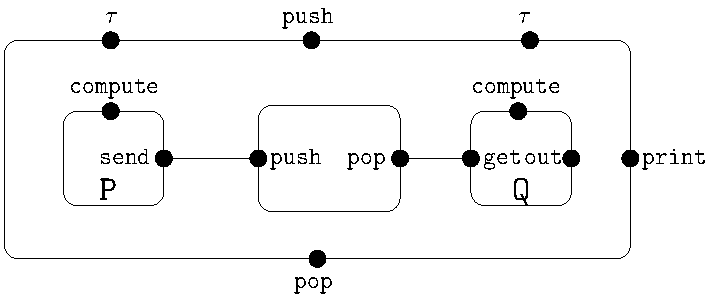
\includegraphics[width=0.8\columnwidth]{figures/Architecture.pdf}
    \caption{Architecture of symbolic model checking}
    \label{architectrue}
\end{figure}



\section{The algorithm}\label{algorithm}

\subsection{Background}

 In \cite{lin1996stga}, Lin presents a symbolic transition graph with assignment (STGA) to model concurrent processes. In a STGA, a node is associated with a set of variables. and the edge between nodes is labelled by guard, assignment and action with a tuple $(b, \bar{x}:=\bar{e}, \alpha)$. The first-order $\mu$-calculus is employed as the property language. In order to check the graph, the first-order $\mu$-calculus is transferred to a graphical version through the proposed rules, and then STGA is checked by the modal graph by the algorithm.
 

 
 \subsubsection{Parameterised action}
From the perspective of syntax, pLTS is similar to STGA. The difference between pLTS and STGA is the $\mathit{action}$. An action in pLTS is a parameterised action $c(args)$. From the syntax of pM$\mu$, we define the parameters in the action as $args$, and $args$ can be one of $!e$, $?x$ and $null$ or the composition of them. While an action in STGA is either a silent action $\tau$, an input action $c?x$, or an output action $c!e$, where $c\in Chan$. 

The difference in parameterised action results in the difference in modality of the algorithm. Based on similarity, we have to change the modality and check the pLTS through the modified algorithm.  

The notation of alternation depth is given by Emerson and Lei in~\cite{emerson1986alternation} as follows:

\textbf{Definition of Alternation Depth}
Given a pM$\mu$ formula $\Phi$, $\Phi_{i}$ is a subformula of $\Phi$ and $\Gamma_{i}$ is a containing fixed point subformula of $\Phi$. The alternation depth $ad(\Phi)$ of $\Phi$ is defined as follows:

\begin{itemize}
\item[-] $ad(A) = ad(X) = 0$, for any atomic proposition $A$ and variable $X$.
\item[-] $ad(\Phi_{1}\wedge\Phi_{2}) = ad(\Phi_{1}\vee\Phi_{2}) = max\{ ad(\Phi_{1}), ad(\Phi_{2})\}$.
\item[-] $ad([\alpha]\Phi) = ad(\langle\alpha\rangle\Phi) = ad(\Phi)$.
\item[-] Let $\sigma\in\{\mu,\nu\}$, and $\bar{\sigma}$ be the dual of $\sigma$. Then
	\begin{center}
	$ad(\sigma X.\Phi) = max\{1, ad(\Phi), 1+ad(\bar{\sigma} X_{1}.\Phi_{1}), ... , 1+ ad(\bar{\sigma} X_{n}.\Phi_{n})\}$
	\end{center} 
	where $\bar{\sigma} X_{1}.\Phi_{1}, ... , \bar{\sigma} X_{n}.\Phi_{n}$ are subpromula of $\Phi$.
\end{itemize}

A formula is said to be alternation-free, when the alternation depth is one, without mutually recursive greatest and least fixed-point operators. In the Timer example, the alternation depth is 1. \TODO{definition of alternation depth]}

 {\color{red}{The order of action and conditional expression???}}
Another difference is the order of action and conditional expression. In pLTS, the order is $<\alpha, e_{b}, (x_{j}:=e_{j})^{j\in J}>$,  and $vars(e_{b})\subseteq vars(s)\cup vars(\alpha)$, and $\forall j\in J. vars(e_{j})\subseteq vars(s)\wedge x_{j}\in vars(s')$. 

While it is $< b, \bar{x}=\bar{e}, \alpha>$ in STGA.


\subsection{Abstract data domain}

In a pLTS, the parameterised action $start(?M)$ includes a parameter in it, and whether the parameter is a variable or a constant is unknown at the abstract level. Abstract values are associated with parameters instead of concrete values \cite{cousot1976static}. We use a symbolic interpretation on parameters $M$. 


\TODO{
In order to construct the abstract data domains, we divide the value of $Max$ to variable and constant. If Max is a variable, Max can express the interval on integer. The change of the value is controlled by a self-decreasing operator. Also, we need another integer 0 as the minimal boundary. If Max is a constant, i.e. Max is the maximal boundary and 0 is the minimal boundary. So we need another variable $pos$ as the interval between Max and 0. Fig.~\ref{side:a} and Fig.~\ref{side:b} are two interpretations on the data domain of the variables. Fig.~\ref{side:a} shows an interpretation that includes two constant (Max, 0), a variable (pos) and an operator (-) on the integer. While Fig.~\ref{side:b} specifies that $Max$ is a variable.
}


\begin{figure}[htbp]

	\begin{tikzpicture}[->, shorten >=2pt, >=stealth, node distance=1.5cm,
	noname/.style={ellipse, minimum width=2.5em, minimum height=1.5em,draw}]
	\node[noname] (1)                                             {$Max$};
	\node[noname] (2) [node distance=0.5cm and 2cm, above right=of 1]                                {$0$};
	\node[noname] (3) [node distance=0.5cm and 2cm, below right=of 1]                                {$pos$};
	
	\path 	(1) edge                   	node[above] {$-$} (2)
	(1) edge                   	node[above] {$-$} (3)
	(3) edge                   node[right] {$-$} (2);
	\path[->] (3) edge [in=-10,out=20,loop] coordinate[pos=0.52] (midp) node[right] {$-$} (3);
	\end{tikzpicture}
	\caption{Interpretation on $Max$}   \label{side:a}

\end{figure}



\subsection{The algorithm for checking pLTS}


\subsubsection{Processing parameterised action}
We change the algorithm to make it suitable for checking pLTS. From the syntax of pM$\mu$, we define the parameters in the action as $args$, and $args$ can be one of $!e$, $?x$ and $null$ or the composition of them. In the modification version, we change the modality from $[c!e], \langle c!e\rangle$, $[c?x], \langle c?x\rangle$ to $[c]$, $\langle c\rangle$, $[c(args)], \langle c(args)\rangle$.
It was shown as follows:

$[c]\Rightarrow$ $checkAnd(\{ (p_{i}, (n', \rho))\,|\, p \xrightarrow{c} p_{i}, n\rightarrow n' \})$
		
$\langle c\rangle\Rightarrow$ 
	 $checkOr(\{ (p_{i}, (n',\rho))\,|, p \xrightarrow{c} p_{i}, n \rightarrow n'\})$
		
$[c(?x, !e)]\Rightarrow$
	$ checkAnd(\{ (p_{i}[v/y], (n',\rho\{x \rightarrow v\}))\,|\,  n \rightarrow n', p \xrightarrow{c(?y, !\rho(e)) } p_{i},v\in Val\})$
		
{$\langle c(?x, !e)\rangle\Rightarrow$}
	 $ checkOr(\{ (p_{i}[v/y], (n', \rho\{x \rightarrow v\}))\,|\,  n \rightarrow n', p \xrightarrow{c(?y, !\rho(e))} p_{i},v\in Val\})$
		
The full algorithm can be seen in the appendix.

\subsubsection{Processing alternation-free pM$\mu$}
The formula in pM$\mu$ is alternation-free, so the alternation depth is 1 in each node of pMG. In the model checking graph, we don't need to use recursion, and the function $restore(D, b)$ in the algorithm is useless for checking pLTS.

\TODO{The principle of model checking}
Given a pLTS model $M$ and a pM$\mu$ $f$, the algorithm checks whether the model satisfies the formula $M\models f$. First, the pM$\mu$ is transferred to a pMG. As for the compositional model checking graph of pMG and pLTS, each state is made up with a couple $\{s\rho, n\rho'\}$, where $s$ is a state in pLTS, and $n$ a node of pMG. A transition of the model checking graph is from $\{s\rho, n\rho_{0}\}$ to $\{s'\rho', n'\rho_{0}'\}$.  The label of the transition is the same as that of pLTS, and the label of the state is the same as that of the node in pMG.



\subsection{The execution result}

After running the algorithm in the appendix, the model checking graph is shown in Fig.~\ref{checkinggraph}:


\begin{figure}
	\begin{tikzpicture}[->, shorten >=2pt, >=stealth, node distance=2cm,
	noname/.style={ellipse, minimum width=3em, minimum height=1.5em, draw}]
	\node[noname] (1)                                             {$S_{0}$};
	\node[noname] (10) [node distance=0.5cm and 2cm, above right=of 1]                                {$S_{10}$};
	\node[noname] (11) [node distance=0.5cm and 2cm, below right=of 1]                                {$S_{11}$};
	\node[noname] (20) [node distance=0.5cm and 2cm, above right=of 10]                                {$S_{20}$};
	\node[noname] (30) [node distance=0.5cm and 2cm, above right=of 20]                                {$S_{30}$};
	\node[noname] (31) [node distance=0.5cm and 2cm, below right=of 20]                                {$S_{31}$};
	\node[noname] (40) [right=of 30]                                {$S_{40}$};
	
	
	\node[noname] (21) [node distance=0.5cm and 2cm, below right=of 11]                                {$S_{21}$};
	\node[noname] (32) [node distance=0.5cm and 2cm, above right=of 21]                                {$S_{32}$};
	\node[noname] (33) [node distance=0.5cm and 2cm, below right=of 21]                                {$S_{33}$};
	\node[noname] (41) [right=of 32]                                {$S_{41}$};
	
	
	\path 	(1) edge                   	node[above] {$\langle start?M\rangle,1$} (10)
	(1) edge                   	node[above] {$\langle start?M\rangle,1$} (11)
	(10) edge                   node[above] {${\mu},1$} (20)
	(20) edge                 	node[above] {$\vee,1$} (30)
	(20) edge                 	node[above] {$\vee,1$} (31)
	(31) edge [bend left] 			node[below] {$\langle true\rangle,1$} (20)
	(30) edge               	node[above] {$\langle timeout\rangle,1$} (40)
	
	
	(11) edge                   node[above] {${\mu},1$} (21)
	(21) edge                 	node[above] {$\vee,1$} (32)
	(21) edge                 	node[above] {$\vee,1$} (33)
	(33) edge [bend left] 			node[below] {$\langle true\rangle,1$} (21)
	(32) edge               	node[above] {$\langle timeout\rangle,1$} (41);
	
	\end{tikzpicture}
	\caption{Model checking Graph}
	\label{checkinggraph}
\end{figure}
where:
\begin{itemize}
	\item $S_{0}  = (\{s_{0},s_{[\rho=\emptyset]}\}, \{n_{1}, \rho_{0}'=\emptyset\}\;|\;s.\sigma = false)$
	\item $S_{10} = (\{s_{1},s_{[t\leftarrow 0]}\}, \{n_{2}, \rho_{0}'(M\leftarrow 0)\}\;|\;s.\sigma = false)$
	\item $S_{20} = (\{s_{1},s_{[t\leftarrow pos]}\}, \{n_{3}, \rho_{0}'(t\leftarrow n_{2})\}\;|\;s.\sigma = false)$
	\item $S_{30} = (\{s_{1},s_{[t\leftarrow 0]}\}, \{n_{4}, \rho_{0}'(t\leftarrow 0)\}\;|\;s.\sigma = false)$
	\item $S_{31} = (\{s_{1},s_{[t\leftarrow 0]}\}, \{n_{5}, \rho_{0}'(t\leftarrow 0)\}\;|\;s.\sigma = false)$
	\item $S_{40} = (\{s_{0},s_{\rho[true]}\}, \{n_{6}, \rho_{0}'(true)\}\;|\;s.\sigma = true)$
	
	\item $S_{11} = (\{s_{1},s_{[t\leftarrow pos]}\}, \{n_{2}, \rho_{0}'(M\leftarrow pos)\}\;|\;s.\sigma = false)$
	\item $S_{21} = (\{s_{1},s_{[t\leftarrow pos]}\}, \{n_{3}, \rho_{0}'(t\leftarrow n_{2})\}\;|\;s.\sigma = false)$
	\item $S_{32} = (\{s_{1},s_{[t\leftarrow 0]}\}, \{n_{4}, \rho_{0}'(t\leftarrow 0)\}\;|\;s.\sigma = false)$
	\item $S_{33} = (\{s_{1},s_{\rho[t\leftarrow t-1]}\}, \{n_{5}, \rho_{0}'(t\leftarrow t-1)\}\;|\;s.\sigma = false)$
	\item $S_{41} = (\{s_{0},s_{\rho[true]}\}, \{n_{6}, \rho_{0}'(true)\}\;|\;s.\sigma = true)$
	\item $n_{2}'=\mu X(pos/t)(\langle timeout\rangle true \vee \langle true\rangle X(pos-1))$
	\item $n_{3}=\langle timeout\rangle true \vee\langle true\rangle\mu X(pos)(\langle timeout\rangle true \vee \langle true\rangle X(pos-1))$
\end{itemize}

In the initial state, there is no variable for the pLTS. After the action $start(?M)$ triggers the transition from $s_{0}$ to $s_{1}$, the value of the variable $t$ will be changed to $Max$. In the transition, the action expression of the operator in the edge of pMG will trigger the occurrence of transitions in pLTS. The change of value in $s$ depends on the semantics of pLTS. In the state $s_{1}$, the system will check whether the guard $t>0$ satisfies. If yes, the action $tick$ will lead to the occurrence of loop transition. Or, the system will enter another transition back to the initial state $s_{0}$. \TODO{After executing the model checking graph, it will finally return to state $S_{40}$ or state $S_{41}$. Both of them are true.}



\section{Checking open automata}



\subsection{Open Automata}



\begin{definition}[pNets]\label{def-pnets}
A pNet is a hierarchical structure where leaves are pLTSs and holes\footnote{Typing can 
be added to pNets by defining and checking their interfaces, called 
sort~\cite{HMZ-FORTE2016}}:
$\pNet\triangleq \pLTS~|~\mylangle \pNet_i^{i\in I}, J, \symb{SV}_k^{k\in 
K}\myrangle$
where
\begin{itemize}
\item[$\bullet$] $\pNet_i^{i\in I}$ is the family of sub-pNets;
%  $\pNet_i^{i\in I}$ is a family of sub-pNets where $I\in\I_\P$ is the set over which 
%sub-pNets are indexed.

\item[$\bullet$] $J$ is a set of indexes, called \emph{holes}.
$I$ and $J$ are \emph{disjoint}: $I\!\cap\! J=\emptyset$,  $I\!\cup\! J\neq\emptyset$
%\item[$\bullet$] $\Sort_j \subseteq \AlgAS$ is a set of action terms, denoting the 
%\emph{sort} of
%hole $j$.

\item[$\bullet$] $\symb{SV}_k^{k\in K}$ is a set of
  synchronisation vectors. % (\hl{$K\in\I_\P$}). 
$\forall k\!\in\! K,
  \symb{SV}_k\!=\SV{\!\alpha_{l}^{l\in I_k \uplus J_k}}{\alpha'_k}{g_k}$, where
  $\alpha'_k\in \actions{\variables}$, $I_k\subseteq I$, $J_k\subseteq J$, and 
  $\vars(\alpha'_k)\subseteq \bigcup_{l\in I_k\uplus 
  J_k}{\vars({\alpha_l})}$. The global action of a vector $\symb{SV}_k$ is
$\alpha'_k$. The Boolean expression $g_k $, such that $\vars(g_k)\subseteq \bigcup_{l\in 
I_k\uplus J_k}{\vars({\alpha_l})}$, is a guard associated to the vector.


\end{itemize}
We define the set of holes and leaves of a pNet as follows:
  \begin{itemize}
\item
The set of holes $\Holes(\pNet_{i_1})$ of a pNet is the indexes of the holes of the pNet 
itself plus the indexes of all the holes of its subnets (we suppose those indexes 
disjoints).
%
%defined inductively; the sets of holes
%in a pNet node and its subnets are all disjoint:
%  \[\begin{array}{l}
%\Holes(\mylangle S,s_0, \to\myrangle) \!=\! \emptyset \\
%\Holes(\mylangle \pNet_i^{i\in I}\!,\Sort_j^{j\in J}\!, \overline{\symb{SV}}\myrangle) 
%=J\uplus{\displaystyle \bigcup_{i\in 
%I}\Holes(\pNet_i)}\\
%\forall i\in I.\, \Holes(\pNet_i)\cap J=\emptyset\\
%\forall i_1,i_2\in I.\,i_1\neq i_2\Rightarrow  
%\Holes(\pNet_{i_1})\cap\Holes(\pNet_{i_2})=\emptyset
%\end{array}\]
\item
The set of leaves of a pNet is the set of all pLTSs occurring in the structure, as an 
indexed family of the form $\Leaves(\pNet)= \mylangle \pNet_i \myrangle^{i \in L}$.
is said to be \emph{open}.
\end{itemize}
A pNet $Q$ is \emph{closed} if it has no hole: $\Holes(Q)=\emptyset$; else it
is said to be \emph{open}.
\end{definition}



The semantics of open pNets will be defined  as an open automaton. An open
automaton is an automaton where each transition composes transitions of several LTSs with action of some holes, the transition occurs if some predicates hold, and can involve a set of state modifications.

\begin{definition}[Open transitions]
	\label{def:OpenTransitions}
	An \emph{open transition} over a
	set $J$ of holes  and a set of states $\mathcal{S}$ is 
	a structure of the form:	
	\begin{mathpar}
	\inferrule*[myfraction=\reddottedrule]
	{	\beta_j^{j\in J}, \Pred, \Post}
	{s \OTarrow {{\alpha}}s'}
	\end{mathpar}
	Where $s, s'\in\mathcal{S}$ and $\beta_j\in\actions{\variables}$
        is an action of the hole $j$. $v$ is a variable denoting the resulting action
        of this open transition. \Pred\ is a predicate 
	over the different variables of the
	terms, labels, and states  $\beta_j$, $s$, $\alpha$. $\Post\in 
	\assigns{\variables}$\ is 
	a set of assignments that are the effects of the transition.
Open transitions are identified modulo logical equivalence on their predicate.
\end{definition}


\begin{definition}[Open automaton]
	\label{def:open-automaton}
	An \emph{open automaton} is a structure\\ $A =
	<J,\mathcal{S},s_0,\mathcal{T}>$ where:
	\begin{itemize}
		\item[$\bullet$]  $I$ and $J$ are  sets of indices,
		\item[$\bullet$]   $\mathcal{S}$ is a set of states and $s_0$ an initial state
		among $\mathcal{S}$,
		\item[$\bullet$] $\mathcal{T}$ is a set of open transitions and for each
		$t\in \mathcal{T}$ there exist $I'$, $J'$ with $I'\subseteq I$, $J'
		\subseteq J$, such that $t$ is an open transition over $J'$,
		and  $\mathcal{S}$.
		
	\end{itemize}
\end{definition}
	

\begin{definition}[States of open pNets]\label{def-states}
  A state of an open pNet is a tuple (not necessarily finite) of the
  states of its leaves.

  For any pNet p, let $\Leaves(p) = \mylangle S_i,{s_i}_0, \to_i\myrangle^{i \in L}$ be 
  the set of pLTS at its leaves,
  then $States(p) = \{\triangleleft s_i^{i\in L}
  \triangleright| \forall i\in L. s_i \in S_i\}$.
A pLTS being its own single leave:
  $States(\mylangle S,s_0, \to\myrangle) = \{\triangleleft s \triangleright| s \in S\}$.

The initial state is defined as:
$InitState(p) = \triangleleft {{s_i}_0}^{i\in L}  \triangleright$.
\end{definition}

\paragraph{Predicates:}
Let
$\mylangle\overline{\pNet},\overline{\Sort},\overline{\symb{SV}}\myrangle$
be a pNet. Consider a synchronisation vector $\symb{SV}\in \overline{\symb{SV}}$. We 
define a
predicate $\Pred$ relating
the actions of the involved sub-pNets and the resulting actions. This predicate verifies:
\begin{multline}
\Pred_{\symb{sv}}(\SV{{(\alpha'_i)}^{i\in I}, {(\beta'_j)}^{j\in J}} 
{\alpha'} {g}, \alpha_i^{i\in I}, \beta_j^{j\in J}, \alpha)\Leftrightarrow \\
\forall i\in I.\, \alpha_i=\alpha'_i\land \forall j \in J.\, \beta_j=\beta'_j \land 
\alpha=\alpha' 
\land g
\end{multline}


 In any other case (if the action families do not match or if there is no valuation of variables such that the above formula can be ensured) the predicate is undefined.

This definition is not constructive but it is easy to build the predicate constructively by brute-force unification of the sub-pNets actions with the corresponding vector actions, possibly followed by a simplification step.

 

 \subsection{The difference between pLTS and open automaton}
 pLTS is a labelling transition system with parameterised action. An open pNet is a composition of some pLTSs and some holes, and a set of synchronization vector composites the action of an open pNet. A BIP architecture of an open pNet includes coordinator components and some operand components. An open automaton is formed by the unfolding of an open pNet through the rules in~\cite{xudong2017smt}. 
 
 In order to check the model of open automata, the algorithm in the appendix have to be modified. There are two different things in the structure of open automaton and pLTS.
 \subsubsection{Hole}
 A hole in pNet is defined without states, but it involves in a transition, which is defined as $\{\xrightarrow{b_j}_j\}^{j\in J}$. The action $b_{j}$ is the action of a hole with an index $j$. The difference of holes from pLTS is whether a component involves in a set of states. However, each action in the hole belongs to a set of the parameterised action.
 
 
 
 \subsubsection{Predicate}
 A transition in a pLTS is consisted of a tuple with labelling $guard$, $parameterised\; action$, $assignment$ between two states. Formally, a transition is defined as $s\xrightarrow{\langle\alpha, e_{b}, (x_{j}:=e_{j})^{j\in J}\rangle}s'$. While an open transition in an open automaton is defined with labelling $Pred$ and $Post$ between a composition of states in pLTSs and holes. In the open transition, $Pred$ is a predicate over the different variables of the terms, labels, and states. Specifically, a predicate consists of a set of parameterised actions in pLTSs and actions in holes. \NOTE{In a pNet, some ports from each component have an immediate relationship, and these ports are connected each other. Also, one of these ports is treated as a action to trigger a transition in the pLTS or in a hole. A predicate is a synchronization vector from the action in each pLTS and each hole.}
 
\subsection{opM$\mu$}
In order to check open automata, a new property language is present. The property language is called open parameterised modal $\mu$-calculus (opM$\mu$). We give the syntax in Tab.~\ref{opmu}:

\begin{table}
	%	\multirow{2}{*}{Algorithme}
	\setlength\tabcolsep{18pt}% default value is 6pt 
	\centering 
	\caption{Syntax of the opM$\mu$} \label{opmu}
	\begin{tabular}{>{\bfseries}c| c } 
		\hline 		
	Action formula of pLTS &     $\alpha ::= \{c(arg_{1}, ..., arg_{n})\mid arg_{i}=?x\mid\ !e\mid \tau\}$                  \\
	& $|\ \neg\alpha \ |\ \alpha_{1}\vee\alpha_{2}\ |\ \alpha_{1}\wedge\alpha_{2}$   \\ 	\hline 
	
	Action formula of Hole &     $\beta ::= \{c(arg_{1}, ..., arg_{n})\mid arg_{j}=?x\mid\ !e\mid \tau\}$                  \\
	& $|\ \neg\beta \ |\ \beta_{1}\vee\beta_{2}\ |\ \beta_{1}\wedge\beta_{2}$   \\ 	\hline 

	Action formula of pNet &     $\gamma ::= \{c\}\ |\ \neg\gamma \ |\ \gamma_{1}\vee\gamma_{2}\ |\ \gamma_{1}\wedge\gamma_{2}$   \\ 	\hline 		
		
	Predicate &     $pred ::= \alpha\wedge \beta\wedge \gamma$   \\ 	\hline 
		
	 	&  $\varphi ::= p \mid X \mid \neg\varphi \mid \varphi_{1}\wedge\varphi_{2}\ |\ \varphi_{1}\vee\varphi_{2} $\\
	 State formula & $\ |\ [\alpha]\varphi \ |\ \langle\alpha\rangle\varphi \ |\ [\beta]\varphi \ |\ \langle\beta\rangle\varphi \ |\ [\gamma]\varphi \ |\ \langle\gamma\rangle\varphi $  \\ 
	& $\ |\ \exists x_{i}\varphi\ |\ \forall x_{i}\varphi\ |\ \mu X(e_{i}/x_{i})\varphi\ |\ \nu X(e_{i}/x_{i})\varphi$	\\ \hline 
	\end{tabular} 
\end{table} 

\TODO{One thing is how to distinguish the action of pLTSs, Holes and pNet, i.e. whose action does $\langle resume\rangle$ stand for?}

An opM$\mu$ is defines as a property language that is used to describe the concurrent systems. $\alpha$ is an action formula from pLTS. $\beta$ is a Hole action formula. $\beta$ can be a $c(arg_i)$ with three kinds of parameter $?x, !e, \tau$,  or the composition of several $\beta$ formula with negation, disjunction and conjunction. $\gamma$ is an action formula from open transition, and it is defined as an action name or the negation of $gamma$, or the disjunction and conjunction of two $\gamma$ formula. A predicate, which is the disjunction of $\alpha$, $\beta$ and $\gamma$, labels an open transition. In the state formula, $[\beta]\varphi$, $\langle\beta\rangle\varphi$, $[\gamma]\varphi$ and $\langle\gamma\rangle\varphi$ are added into the list.

An example of opM$\mu$ is employed to the formula for open automaton in Sec.~\ref{Sec2:usecase}.  The formula can be expressed as follows:
\begin{equation}\label{formula3}
	\langle fail?M\rangle \mu X(t).\langle finish\rangle true \vee (\langle reset\vee resume\rangle true \vee \langle tick\rangle X(t-1))
\end{equation}

If a $fail$ occurs with receiving a value $M$, and then a $finish$ happens only after a $resume$ or $reset$ occurs after $M$ times $tick happens$ with decreasing $t$ by one. The formula can be employed to express that an action $finish$ always eventually happens until the $reset$ or $resume$ occurs after the loop $tick$ happens.

If we describe the Formula.~\ref{formula3} with a graphical pMG, it can be shown as Fig.~\ref{pmg3}:


\begin{figure}
\centering
	\begin{tikzpicture}[->, shorten >=2pt, >=stealth, node distance=1.2cm,
	noname/.style={ellipse, minimum width=1.5em, minimum height=1.5em, draw}]
	\node[noname] (1)                                            				 	{$t_{1}$};
	\node[noname] (2) [right=of 1]                               				 	{$t_{2}$};
	\node[noname] (3) [right=of 2]                              				 	{$t_{3}$};
	\node[noname] (4) [node distance=0.5cm and 2cm, above right=of 3]    {$t_{4}$};
	\node[noname] (5) [right=of 4]                                					{$t_{5}$};
	\node[noname] (6) [node distance=0.5cm and 1.8cm, below right=of 3]     {$t_{6}$};
	\node[noname] (7) [node distance=0.4cm and 1.8cm, above right=of 6]     {$t_{7}$};
	\node[noname] (8) [right=of 7]     {$t_{8}$};
	\node[noname] (9) [node distance=0.4cm and 1.8cm, below right=of 6]     {$t_{9}$};

	
	\path 	(1) edge                   	node[above] {} (2)
	(2) edge                   	node[above] {} (3)
	(3) edge 			node[above] {} (4)
	(3) edge 			node[above] {} (6)
	(9) edge[bend left]    node[below] {} (3)
	(4) edge    		node[below] {} (5)
	(6) edge    		node[below] {} (7)
	(7) edge    		node[below] {} (8)
	(6) edge    		node[below] {} (9);


	\end{tikzpicture}
	\caption{The associated pMG of Formula~\ref{formula3}}\label{pmg3}
\end{figure}

where:
\begin{itemize}
	\item $L_{N}(t_{1}) = (\{\}, \langle start?M\rangle, 1)$
	\item $L_{N}(t_{2}) = (\{t\}, t := M, 1)$
	\item $L_{N}(t_{3}) = (\{t\}, \vee, 1)$
	\item $L_{N}(t_{4}) = (\{t\}, \langle finish\rangle, 1)$
	\item $L_{N}(t_{5}) = (\{\}, true, 1)$
	\item $L_{N}(t_{6}) = (\{t\}, \vee, 1)$
	\item $L_{N}(t_{7}) = (\{t\}, \langle resume \vee reset\rangle, 1)$
	\item $L_{N}(t_{8}) = (\{\}, true, 1)$
	\item $L_{N}(t_{9}) = (\{t\}, \langle tick\rangle, 1)$
\end{itemize}

\NOTE{Explain the graph}



\subsection{The modified algorithm}

An open automaton is unfolded by a pNet with some pLTSs and holes. An open transition is defined by a hole action, a predicate, a postcondition, and a transition labelled by a synchronisation vector between a composition of states from different pLTSs. 

What we have to deal with in the algorithm is the $hole$ and $predicate$. 


\section{Related work}

\section{ Conclusion}



\section*{Appendix}

\algnewcommand\algorithmicswitch{\textbf{switch}}
\algnewcommand\algorithmiccase{\textbf{case}}
\algnewcommand\algorithmicassert{\texttt{assert}}
\algnewcommand\Assert[1]{\State \algorithmicassert(#1)}%
% New "environments"
\algdef{SE}[SWITCH]{Switch}{EndSwitch}[1]{\algorithmicswitch\ #1\ \algorithmicdo}{\algorithmicend\ \algorithmicswitch}%
\algdef{SE}[CASE]{Case}{EndCase}[1]{\algorithmiccase\ #1}{\algorithmicend\ \algorithmiccase}%
\algtext*{EndSwitch}%
\algtext*{EndCase}%

\begin{algorithm} 
	\begin{algorithmic}[1]
		\State stack[0 ... (k-l)]
		\State pushStack(s) = push s onto stack[s.depth]
		\State top() = return the top element of the first non-empty stack with the deepest depth
		\State pop() = remove from the stack the element returned by the last call to top 
		\State $s=\{s.depth, s.status, s.\sigma, s.D, s.instack\}$
		\State modelCheck(s) = \{ s.status := VISITED($s.\sigma)$; push(s);
		\While{stack is non-empty}
		\State close(top()); \Return s.status; \}
		\EndWhile
		
	\end{algorithmic} 
	\caption{modelCheck(s)}
	\label{alg:algorithm1}
\end{algorithm}

\begin{algorithm} 
	\begin{algorithmic}[1]
		
		\State close(s as ($p, n\rho'$)) =
		\If{n is root}
		\State $p = m\rho; \rho = \emptyset; \rho' = \emptyset$  
		\EndIf
		\State let checkAnd(W) =
		\State let ($B_{i}, D_{i}$) = check($s_{i}$) 
		\For {each $s_{i} \in W$}
		\If {there is some $B_{i}$ = DEFERRED}
		\Return(DEFERRED)
		\ElsIf {there is some $B_{i}$ = VALUE(false)} 
		\State add s to $D_{i}$; \Return(VALUE(false))
		\Else 
		\State add s to each $D_{i}$; \Return(VALUE(true))
		\EndIf
		\EndFor
		\State let checkOr(W) =
		\State let ($B_{i}, D_{i}$) = check($s_{i}$) 
		\For {each $s_{i} \in W$}
		\If {every $B_{i}$ = DEFERRED}
		\Return(DEFERRED)
		\ElsIf{there is some $B_{i}$ = VALUE(true)} 
		\State add s to $D_{i}$; \Return(VALUE(true))
		\Else 
		\State add s to each $D_{i}$; \Return(VALUE(false))
		\EndIf
		\EndFor
		
		
		\State  let $B$ be 
		\Switch{$L_{O}(n)$} 
		\Case{$be$}
		\Return $\rho(be)$
		\EndCase
		\Case{x:=e}
		\Return $checkAnd(\{ (p, (n', \rho\{x\rightarrow \rho(e)\}))\, |\, n \rightarrow n' \})$
		\EndCase
		\Case{$\wedge$} 
		\Return $checkAnd(\{ (p, (n_{i}, \rho))\, n\rightarrow n_{i}\}) $
		\EndCase
		\Case{$\vee$} 
		\Return $checkOr(\{ (p, (n_{i}, \rho))\, n\rightarrow n_{i} \})$
		\EndCase
		\Case{[c]} 
		\Return $checkAnd(\{ (p_{i}, (n', \rho))\,|\, p \xrightarrow{c} p_{i}, n\rightarrow n' \})$
		\EndCase
		\Case{$\langle c\rangle$} 
		\Return $checkOr(\{ (p_{i}, (n',\rho))\,|, p \xrightarrow{c} p_{i}, n \rightarrow n'\})$
		\EndCase
		\Case{[c(?x, !e)]}
		\Return $ checkAnd(\{ (p_{i}[v/y], (n',\rho\{x \rightarrow v\}))\,|\,  n \rightarrow n', p \xrightarrow{c(?y, !\rho(e)) } p_{i},v\in Val\})$
		\EndCase
		\Case{$\langle c(?x, !e)\rangle$}
		\Return $ checkOr(\{ (p_{i}[v/y], (n', \rho\{x \rightarrow v\}))\,|\,  n \rightarrow n', p \xrightarrow{c(?y, !\rho(e))} p_{i},v\in Val\})$
		\EndCase
		\Case{$\forall x$}
		\Return $  checkAnd(\{ (p, (n',\rho\{x \rightarrow v\}))\,|\, n \rightarrow n', v \in Val\})$
		\EndCase
		\Case{$\exists x$}
		\Return $ checkOr(\{ (p, (n',\rho\{x \rightarrow v\}))\,|\,  n \rightarrow n', v\in Val\})$
		\EndCase
		\EndSwitch
		
		\If{B=VALUE(b)}
		\State pop(); 
		\If{s.status = VISITED($b'$) and $b'\neq b$}
		\State s.status = VISITED($b$); 
		\EndIf
		\EndIf
	\end{algorithmic} 
	\caption{$close(s)$}
	\label{alg:algorithm2}
\end{algorithm}	


\begin{algorithm} 
	\begin{algorithmic}[1]
		\State check(s) =
		\Switch{$s.status$}
		\Case{FRESH} 
		\State s.status := VISITED($s.\sigma$); push($s$); \Return (DEFERRED, $s.D$)
		\EndCase
		\Case{VISITED($b$)} 
		\Return (VALUE($b$), $s.D$)
		\EndCase
		\EndSwitch
		
	\end{algorithmic} 
	\caption{check(s)}
	\label{alg:algorithm3}
\end{algorithm}





\begin{thebibliography}{4}
	\bibitem{xudong2017smt}Xudong Qin, Simon Bliudze, Eric Madelaine, Min Zhang. Using SMT engine to generate Symbolic Automata -Extended version. [Research Report] RR-9177, Inria
	
	\bibitem{radu2008mcl}Mateescu, Radu, and Damien Thivolle. "A model checking language for concurrent value-passing systems." International Symposium on Formal Methods. Springer, Berlin, Heidelberg, 2008.
	
	\bibitem{mavridou2016architectrue} Mavridou, Anastasia, et al. "Architecture-based design: A satellite on-board software case study." International Workshop on Formal Aspects of Component Software. Springer, Cham, 2016.
	\bibitem{lin2001modal} Lin, Huimin. "Model checking value-passing processes." apsec. IEEE, 2001.

	\bibitem{lin1996stga} Lin, Huimin. "Symbolic transition graph with assignment." International Conference on Concurrency Theory. Springer, Berlin, Heidelberg, 1996.
	\bibitem{emerson1986alternation}Emerson, E. Allen and Chin-Laung Lei. ?Efficient Model Checking in Fragments of the Propositional Mu-Calculus (Extended Abstract).? LICS (1986).
	\bibitem{cousot1976static}Cousot, Patrick, and Radhia Cousot. "Static determination of dynamic properties of programs." Proceedings of the 2nd International Symposium on Programming, Paris, France. Dunod, 1976.
	
\end{thebibliography}




\end{document}
